\documentclass{beamer} 
\usepackage{multicol}
\usepackage{url}
\usepackage{fancyvrb}
\usepackage{color}
\setbeamercolor{goodcolor}{fg=black,bg=lime}
\setbeamercolor{badcolor}{fg=black,bg=pink}

\title{What every programmer should know about merging branches in Mercurial} 
\author{Sergey Kishchenko} 
\date{\today} 
\usetheme{CambridgeUS}
\usecolortheme{seagull}
\institute{Quickoffice}

\begin{document}

\frame{\titlepage}

\begin{frame} 
\frametitle{Branches}
\begin{multicols}{2}
\center{Two different branches}
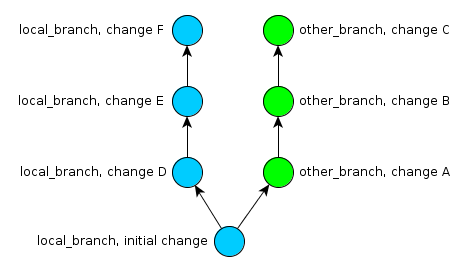
\includegraphics[width=0.4\textwidth]{img/two_branches}
\columnbreak
\center{Two different defaults}
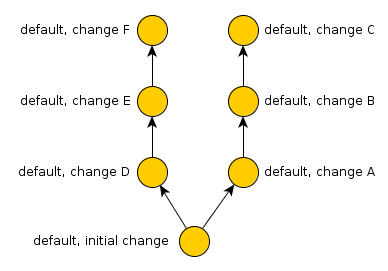
\includegraphics[width=0.4\textwidth]{img/two_default_branches}
\end{multicols}
\begin{itemize}
\item \textbf{NOTE}: Different repos cloned from one source are not actually different, they are more like one repo. You can transfer changes between them with push and pull
\item \textbf{IMPORTANT}: Named branches in Mercurial are permanent!
\end{itemize}
\end{frame}

\begin{frame}[fragile]
\frametitle{Pull}
\begin{exampleblock}{First step in merge process: pulling remote changes}
\begin{verbatim}
> hg pull -b REMOTE_BRANCH REMOTE_REPO
\end{verbatim}
\end{exampleblock}
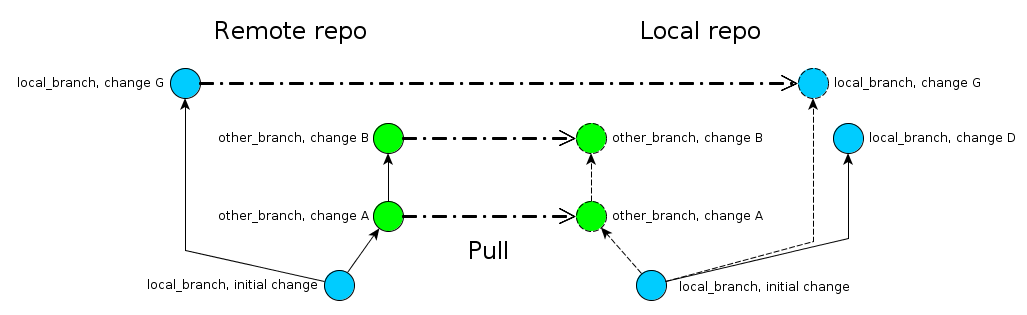
\includegraphics[width=\textwidth]{img/pull_branches}
\begin{itemize}
\item Pulling change pulls also all its ancestors $\to$ unneeded changes
\item Pulling changes may result in creating new heads $\to$ merge is needed
\end{itemize}
\end{frame}

\begin{frame}
\frametitle{Solution attempt: "early-fix" branch}
\begin{multicols}{2}
\center{Bad idea}
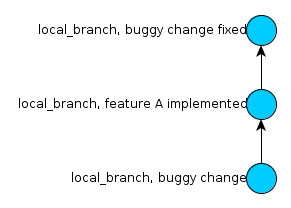
\includegraphics[width=0.4\textwidth]{img/early_fix_branch_bad}
\columnbreak
\center{Good idea}
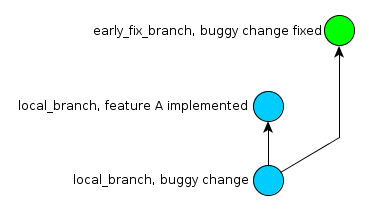
\includegraphics[width=0.4\textwidth]{img/early_fix_branch_good}
\end{multicols}
\begin{beamercolorbox}[rounded=true,center,shadow=true]{goodcolor}
  Having a specific fix branch allows pulling this branch without pulling other changes (Feature A)
\end{beamercolorbox}
\begin{beamercolorbox}[rounded=true,center,shadow=true]{badcolor}
  You should think about it in advance and you're not a psychic
\end{beamercolorbox}
\end{frame}

\begin{frame}
\frametitle{Solution attempt: Patch}
\textbf{IDEA}: Why do we even need to use pull?
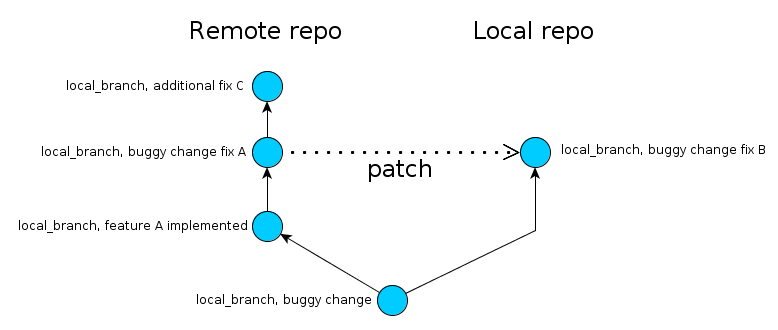
\includegraphics[width=\textwidth]{img/using_patch}

\begin{beamercolorbox}[rounded=true,center,shadow=true]{badcolor}
  Fix A can be based on Feature A so patch will not apply smoothly
\end{beamercolorbox}
\begin{beamercolorbox}[rounded=true,center,shadow=true]{badcolor}
  SCM can't guess that fix A and fix B are actually the same and should be used as base when merging fix C
\end{beamercolorbox}
\end{frame}

\begin{frame}[fragile]
\frametitle{Solution attempt: graft}
\begin{exampleblock}{Using graft}
\begin{verbatim}
> hg graft --log GRAFT_REVISION
\end{verbatim}
\end{exampleblock}
\begin{center}
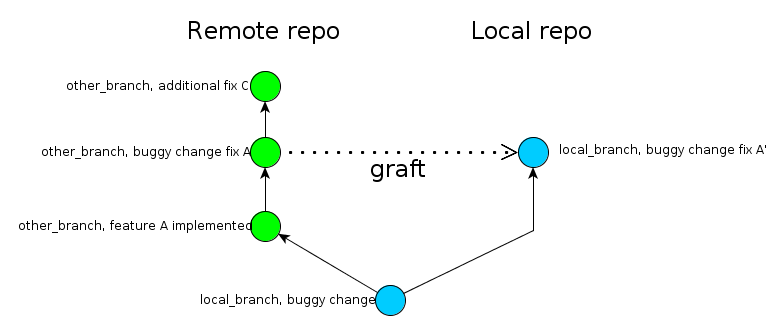
\includegraphics[width=0.8\textwidth]{img/using_graft}
\end{center}

\begin{beamercolorbox}[rounded=true,center,shadow=true]{goodcolor}
  graft uses 3-way merge and deals fine with Fix A being based on Feature A
\end{beamercolorbox}
\begin{beamercolorbox}[rounded=true,center,shadow=true]{badcolor}
  SCM still can't guess that fix A and fix B are actually the same and should be used as base when merging fix C
\end{beamercolorbox}
\end{frame}

\begin{frame}[fragile]
\frametitle{Solution attempt: grafting from remote repo}
\textit{hg graft} doesn't deal with changesets from the remote repo at the moment because it needs all of the changes to do 3-way merge. But it's possible to strip changes when they are not needed anymore
\begin{exampleblock}{grafting from remote repository}
\begin{verbatim}
> hg incoming --template="{node} " REMOTE_REPO -q \ 
    -r GRAFT_REVISION > TEMP_FILE
> hg pull -r GRAFT_REVISION REMOTE_REPO
> hg graft --log GRAFT_REVISION
> hg strip `cat TEMP_FILE`
\end{verbatim}
\end{exampleblock}
\end{frame}

\begin{frame}
\frametitle{Solution attempt: dealing with base issues with graft}
\begin{center}
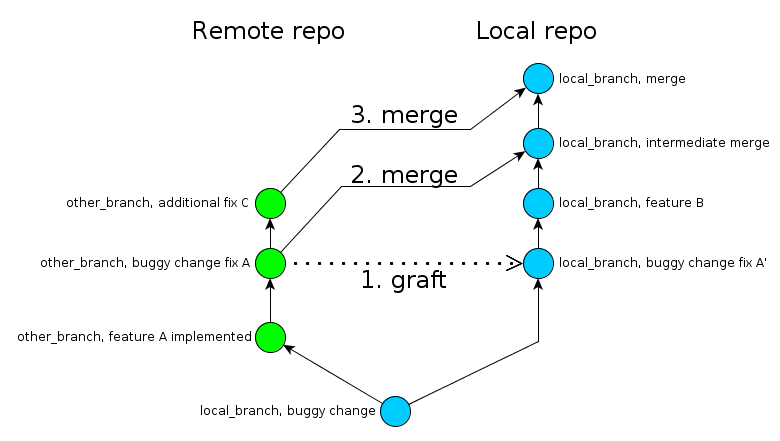
\includegraphics[width=\textwidth]{img/graft_dealing_with_base}
\end{center}
\end{frame}

\begin{frame}[fragile]
\frametitle{Solution attempt: dealing with base issues with graft}
\begin{exampleblock}{Searching for grafted revisions}
\begin{Verbatim}[fontsize=\small]
> hg log -r "ancestor(LOCAL_HEAD,OTHER_HEAD)::LOCAL_HEAD" \
    -k "grafted" -v
e.g.
> hg log -r "ancestor(d5c1ff557965,927d19ecf38e)::d5c1ff557965" \
    -k "grafted" -v
\end{Verbatim}
\end{exampleblock}

\begin{exampleblock}{graft-aware merging}
\begin{verbatim}
> hg merge -R GRAFT_REVISION
> hg merge
\end{verbatim}
\end{exampleblock}
\end{frame}

\begin{frame} 
\frametitle{Solution attempt: Branches alternatives}
\begin{itemize}
\item Bookmarks: \url{http://mercurial.selenic.com/wiki/Bookmarks}
\begin{beamercolorbox}[rounded=true,center,shadow=true, wd=0.9\textwidth]{goodcolor}
Lightweight git-like branches, good for local hacking, distributed along with Mercurial. 
\end{beamercolorbox}
\begin{beamercolorbox}[rounded=true,center,shadow=true, wd=0.9\textwidth]{badcolor}
Several heads on default, no trail in history
\end{beamercolorbox}
\item Local branches, lbranches: \url{http://mercurial.selenic.com/wiki/LocalbranchExtension}. 
\begin{beamercolorbox}[rounded=true,center,shadow=true, wd=0.9\textwidth]{goodcolor}
Lightweight repo clones, good for local hacking
\end{beamercolorbox}
\begin{beamercolorbox}[rounded=true,center,shadow=true, wd=0.9\textwidth]{badcolor}
Just a local feature
\end{beamercolorbox}
\item Patch queues, mq: \url{http://mercurial.selenic.com/wiki/MqExtension} 
\begin{beamercolorbox}[rounded=true,center,shadow=true, wd=0.9\textwidth]{goodcolor}
Patch series, editable history, distributed along with Mercurial
\end{beamercolorbox}
\begin{beamercolorbox}[rounded=true,center,shadow=true, wd=0.9\textwidth]{badcolor}
Just a local feature
\end{beamercolorbox}
\end{itemize}
\end{frame}


\begin{frame}[fragile]
\frametitle{Merge}
\begin{exampleblock}{Naïve approach}
\begin{verbatim}
> hg co local_branch
> hg merge remote_branch
or usually (while in default)
> hg pull 
> hg merge 
\end{verbatim}
\end{exampleblock}
\begin{multicols}{2}
\center{Merging different branches}
Image with merged branches
% \includegraphics[width=0.4\textwidth]{img/delorean-blueprint}
\columnbreak
\center{Merging default}
Image with merged defaults
% \includegraphics[width=0.4\textwidth]{img/delorean}
\end{multicols}
\begin{center}
Isn't always so good :( 
% \includegraphics[width=0.45\textwidth]{img/chubaka}
\end{center}
\end{frame}

\begin{frame}
\frametitle{Probable issues}
\begin{itemize}
\item Too much conflicts
\item Hard to understand the conflict
\item Code was refactored
\item Non-source files conflicts
\end{itemize}
\end{frame}

\begin{frame}
\frametitle{Too much conflicts}
TODO: Why occurs? How to prevent? How to deal with? 
\end{frame}

\begin{frame}
\frametitle{Hard to understand the conflict}
TODO: Why occurs? How to prevent? How to deal with? 
\end{frame}

\begin{frame}
\frametitle{Code was refactored}
TODO: Why occurs? How to prevent? How to deal with? 
\end{frame}

\begin{frame}
\frametitle{Non-source files conflicts}
TODO: Why occurs? How to prevent? How to deal with? 
\end{frame}


\begin{frame}
\frametitle{One more time: good things}
\begin{itemize}
\item Specifying branch for pulling
\item Using graft
\item Using good graphical tool for merging
\item Using 3-way merge
\item Using "early-fix" branches
\item Getting knowledge from others when merging theirs code
\item Providing help to those who merge your code
\item Avoiding unnecessary refactoring when
\end{itemize}
\end{frame}

\begin{frame}
\frametitle{One more time: bad things}
\begin{itemize}
\item Manual merges
\item Applying patches manually
\item Being a coward and selecting one side
\item Trusting automatic merge tools completely
\end{itemize}
\end{frame}

\begin{frame}
\frametitle{One more time: things to avoid}
\begin{itemize}
\item Doing a refactoring that can't be merged into all branches immediately
\item Modifying non-source file without merging it into all branches immediately
\item Modifying a component that somebody is working on without notifying him 
\end{itemize}
\end{frame}


\begin{frame}
\frametitle{Thank you! Questions?}
\begin{center}
% \includegraphics[width=0.45\textwidth]{img/chubaka}
\end{center}
\end{frame}

\end{document}
